%% Comments from editor: 

%% At the end of the piece, there is not really a strong conclusion to
%% finish your narrative. Do you think you could add a sentence or two
%% that would sum things up a bit? Something about the current state of
%% the field, what's up and coming, why things might be looking up, etc?
%% Perhaps something about the fact that there will always be an arms
%% race between criminals and investigators, but new tools hope to make
%% it possible for law enforcement to stay a step ahead? 
%% 
%% Let me know what you think. I'm happy to help in any way possible.
%% 
%% 

\chapter{Introduction}
Over the past decade \emph{digital forensics} (DF) has grown from a trade
practiced by technicians working for law enforcement
organizations and into scientific discipline. Today DF  researchers are
making slow but steady progress on scientifically challenging
problems; DF research is presented at conferences
and published in peer-reviewed journals; and there is a growing
collection of both tools and reference data sets designed to promote
DF education and help validate new research techniques. Because of
both the scale and the diversity of their domain, DF researchers and
practitioners are necessarily at the forefront of some of the most
challenging problems in computer science today, including ``big data''
analysis, natural language processing, visualizations, and
cybersecurity. This article introduces the science of DF research
to those who are not acquainted with the field. 

Broadly construed, DF applies the process and goals of \emph{forensic
  science} to the study of all things digital---and specifically to
digitized information that might be found on computers, cell phones,
storage devices and  computer networks during the course of a
criminal investigation. Compared with traditional ``blood and
bullets'' forensics, DF poses significant challenges for three primary
reasons: information on a computer system can be changed without 
trace; the scale of data that must be analyzed; and the variety of
data types that an investigator can encounter. Just as a traditional forensic investigator must be
prepared to analyze any kind of smear or fragment, no matter the
source, a DF investigator must be able to make sense of any data that
might be found on any digital device anywhere on the planet. In
practice, this is a very difficult proposition.

Much of what we now call DF got its start in the 1980s
as computer systems were increasingly involved in criminal acts.
From its inception, DF served two different
purposes. First, in many cases computers contained evidence of a
crime. In these cases the crime took place in the physical world
and the computer was all but incidental---except for the fact that
computerization made the evidence harder for
investigators to analyze than paper records. For example, Bernard Madoff kept track of
his victims ``accounts'' using an IBM AS/400 minicomputer from the
1980s: the age of the computer  helped perpetuate the crime, since few
people on Wall Street have experience with 25-year-old technology, and
was an added complication to investigators after Madoff was
arrested\cite{technology-madoff}, since investigators had few tools
necessarily to make sense of the data.

The second class of cases are those in
which the crime was inherently one involving computer systems, such as
computer hacking. In these cases, investigators are hampered
by the technical sophistication of the systems and the massive amount
of evidence to analyze.

Today personal computers have become so
ubiquitous that the collection and use of computerized evidence is no
longer a curiosity---it is now a part of many criminal and civil
investigations. Suspects in murder cases now routinely have their
laptops and cell phones examined for corroborating evidence---not
because a computer was the instrument of the crime, but because
computers now mediate so many human-human interactions. 
E-discovery dominates much of today's corporate litigation.

DF is powerful because computer systems are windows into the
past. Many digital systems retain vast quantities of
information---either intentionally, in the form of log files and
archives, or inadvertently, as a result of software that does not
cleanly erase memory and files after it runs. As a result, it
is frequently possible for investigators to recover old email
messages, chat logs,   Google search terms and other kinds of data
that were created
weeks, months, or even years in the past. Such contemporaneous records
can reveal an individual's state-of-mind or intent \emph{at the time
  the crime was being committed}.

But whereas pre-computer evidence such as handwritten letters and
photographs could be photographically reproduced and given to attorneys, judges and juries, computerized evidence
requires special handling and analysis. In part this is because
electronic data are easily changed, damaged or erased if
handled improperly---for example, simply turning on a consumer GPS
may cause the device to erase critical evidence. Additionally,  computers
frequently harbor hidden evidence that may only be evident when
specialized tools are used---for example, a digital camera may appear to have
30 photos, but examination by an expert may reveal that another 300
deleted photos can be recovered.

Because they can look into the past and uncover hidden data,
DF tools are increasingly used beyond the courtroom. Security
professionals use DF tools to analyze network intrusions---not
to convict the attacker, but to understand how the
attacker gained access to plug the hole. Data recovery firms use DF tools to resurrect files from drives that have
been inadvertently formatted or damaged. DF tools can even 
detect the  unintentional disclosures of personal information---for
example, by analyzing computers at the conclusion of a lease to see if
sensitive information remains on their hard drives. For example, in
2009 the Inspector General of the United States Department of Defense
issued a report in which forensic software was used to test hard
drives leaving the government service. The IG found that ``DOD Components did not properly
sanitize, document, or fully account for excess unclassified IT
equipment before it was released to other Federal, DOD, or non-Federal
organizations.''\cite{D-2009-104}

Forensic tools are also used to determine that something did not
happen. Here they are less powerful, for the well known reason that
the absence of evidence is not the evidence of absence. 
For example, in May 2006 a laptop and external hard drive containing
sensitive personal information of 26.5 million veterans and military
personnel was stolen from an employee at the Department of Veterans
Affairs. After the stolen laptop was recovered in June 2006, forensic
investigators analyzed the media and determined that the sensitive
files had probably not been accessed\cite{va-laptop-1}. One way to
make such a determination is by examining the access and modification
times associated with each file on the computer's hard
drive. Of course, the same
forensic techniques that the investigators used could have been
applied to access the VA laptop without modifying those timestamps,
the VA investigators really just determined that the files had not
been asked by convention, non-forensic means.

As the preceding paragraphs make clear, today the field of digital
forensics is largely \emph{tool-based} and
\emph{investigator-centric}. 
That is, the requirements of DF are driven 
by what investigators need to perform digital
investigations\citep{walls-levine-effective-digital-forensics}. Convictions
are frequently the
measure of success. In many cases there is a considerable gap between
what is theoretically possible and what is necessary. That is, even
though there may be an intellectual desire to analyze and explain every last byte
on a piece of subject media\cite{garfinkel:every-last-byte}, there is
rarely a reason to do so.

\section{The Digital Forensics Process and Toolbox}

The tools of digital forensics can be equally applied to suspects,
victims and bystanders. A cell phone found on a dead body without
identification would almost certainly be subjected to analysis, but so
would a phone dropped during a house burglary. For this reason,
discussions of techniques speak about systems under investigation in
abstract terms (e.g. the ``subject computer''). Discussions of
legal issues such as the need for a warrant are separated from
discussions of technology, because different techniques are
permissible in different legal contexts.

Variations in use and policy can be challenging. As the field has
grown, practitioners have tried to create a consistent approach for
performing DF investigation, but the approach must be flexible enough
to cover these different applications. Today we call this approach the
\emph{digital forensic model}. Several such models have been
proposed\citep{pollitt:models}, but most have these common elements:


% http://www.tex.ac.uk/cgi-bin/texfaq2html?label=complist
\subsection{Preparation} 
Before an individual or organization
  performs an investigation, it's important to decide upon the
  standards and procedures that will be followed; to obtain the
  appropriate devices, software, and even cables required for investigations; and to assure that
  investigators and technicians are appropriately trained. In some
  cases preparation may take years, requiring 
  certification of forensic laboratories and the formal testing of
  tools to determine their effectiveness and error rates. 

  When it comes to preparation, two important tools are the American Society of Crime Laboratory
  Directors/Laboratory Accreditation Board (ASCLD/LAB) laboratory
  accreditation program and individual examiner certification programs such as
  the Certified Computer Examiner.

\subsection{Collection and Preservation} 
Before data can be analyzed, they
  are taken from the field (the ``scene of the crime''),
  stabilized and preserved to create a lasting record. 

  Although digital computers are based entirely on computations
  involving the binary digits 0 and 1, more commonly known as
  \emph{bits}, modern computers do most of their work on groups of
  eight bits called \emph{bytes}. Because each binary digit can be a 0
  or a 1, a byte can represent the numbers $00000000$, $00000001$,
  $00000010$, $\ldots$ $11111111$, or the decimal numbers 0 through
  255 (recall that $2^8=256$). When working with digital forensics,
  it's common to use hexadecimal representation (base 16), which
  represents these are the numbers \texttt{00} through \texttt{FF}
  ($15\times16+15=255$).

  One common use for bytes inside the computer is to store written
  text. To store text, each letter is represented by a specific binary
  code. UTF-8, a common representation in use today, uses the
  binary sequence 00100001 (hexdecimal \texttt{41}) to represent the
  letter A, 00100010 (\texttt{42}) for the letter
  B. 
\includegraphics{uni/unicode_547d} is the Han ideograph
  representing life; it has the hexdecimal coding \texttt{547D}. 

When recorded on a hard drive or camera card, these bytes are groups in
  blocks called \emph{sectors} that are typically 512 or 4096 bytes in
  length. A sector is the smallest block of data that a drive can read
  or write. An email message might require 10 or 20 sectors to
  store; a movie might require hundreds of thousands. Depending on the
  arrangement of other files on the device, the sectors can be stored
  as a single sequential stream or they can be fragmented into many
  different locations. Other sectors contain information that the
  computer uses to find the stored information: such bookkeeping
  information is called ``file system metadata.''

  Each sector on the disk has a unique identifying number, called
  the sector's \emph{logical block address} (LBA). An Android phone
  advertised as having ``8GB'' of storage has eight billion bytes or roughly 15
  million sectors.  To preserve the data on a computer or phone, each of these sectors
  must be individually copied out of the phone or off the hard drive and
  stored on another computer in a single file called a \emph{disk image}
  or \emph{physical image}. This file, which contains every single byte
  stored on the target device, naturally includes every
  visible file on the media. But the physical image also records
  invisible files as well as portions of files that have been deleted
  but not yet overwritten by the operating system. 

  For typical desktop or laptop computers, collection and preservation
  is performed with a program called a \emph{disk imager}, of which there
  are many. Disk imager  are tested by the Computer Forensic
  Tool Testing Program (CFTTP) at the National Institute of Standards and
  Technology (NIST) Information Technology Lab (ITL) to make sure that
  they accurately copy all of the data off the subject
  device. Although it might seem straightforward, the task is
  complicated by the possible presence of bad sectors and ``hidden''
  storage, the need for the program to detect and accurately report
  the drive being unplugged, and other issues that may seem
  inconsequential but which can be very significant when a disk image
  is being used as the basis of a criminal prosecution. 

  In the case of network forensics, it is the actual data
  sent over the network connection that are preserved. This means that network forensics
  equivalent to a wiretap---and in fact network forensics equipment is
  increasingly used for wiretaps by law enforcement. 

%  Today's computer networks carry information in blocks
%  called \emph{packets} which are typically between 50 and 1500 bytes
%  in length. Network collection is performed with tools called
%  \emph{packet sniffers} or \emph{network forensic analysis tools}
%  (NFATs)\cite{613756}. These tools intercept the packets that are
%  sent down a wire (or through the air) and copy them into a file
%  called a ``packet trace'' or a ``PCAP'' (packet capture) file.  

  Increasingly the random access memory (RAM) associated with computer
  systems is also being subjected to forensic investigation. RAM is
  difficult to work with, as it changes very quickly and is lost when
  a computer is turned off. RAM must also be captured with a special
  program (a ``memory imager'') and is stored in its own special kind
  of file called a ``memory dump.'' Although memory can be extracted from all
  kinds of computer systems, including desktops, laptops, cell phones,
  as well as network communications equipment such as wireless
  routers, each of these systems uses different kinds of internal
  structures, so software designed to analyze one may not analyze another.

  Although forensics researchers have developed approaches for
  assuring the forensic integrity of drive copies, currently there is
  no widely accepted approach for mathematically assuring a RAM dump.

\subsection{Examination and Extraction} Working with the preserved data, an
  examiner will explore for any information that might be
  relevant to the investigation at hand. 

  When performing disk forensics, files that can be seen from within
  the computer's own operating system are called ``allocated files''
  because the storage associated with the files is allocated to that
  purpose. On many system it is also possible to recover files that have
  been deleted but whose previously allocated sectors have not yet
  been overwritten or otherwise used for another purpose. These
  sectors are said to contain \emph{deleted files}, \emph{residual data}, or
  \emph{digital trace evidence}.

Most examinations are performed
  with tools that can extract user files from the disk image, search for files that contain a specific word or phrase
  in a variety of human languages, and even detect the presence of
  encrypted data. One common technique is to arrange all of the
  information chronologically and create a timeline that shows when
  each file on the disk was modified or last accessed. Another 
  technique is to review every directory and file and look for
  things that seem out-of-the-ordinary. Relevant data are then
  extracted from the preserved system so that they are easier to
  analyze---for example, an individual file may be sent to a linguist
  for translation. In the military this process of examination and extraction
  is frequently called \emph{exploitation}.

  There are many tools for performing examination. The Sleuth Kit\cite{sleuthkit} is
  an open source tool that can decode Windows, Macintosh, Linux, XBox,
  and Android
  file systems, recovering both allocated and deleted
  files;   Volatility\cite{volatility} can analyzing memory dumps from a
  variety of different systems.

\subsection{Analysis} Once potentially relevant information is
  extracted, an analyst will construct one or more hypotheses that
  uses the digital evidence to explain possible past activities. A
  hypothesis may draw from multiple digital devices---an email message
  sent from a desktop computer to a cell phone, for example---or the
  hypothesis may incorporate events in the physical world, like a
  power failure or theft. During this phase a good analyst will also
  try to construct alternative hypotheses that are consistent with the
  evidence but which point to different conclusions. In Europe it is
  popular for examiners to perform an Bayesian analysis and estimate
  the probability of each hypothesis based on the available data.

  Many examination tools can perform some kind of analysis, but there
  are also commercial tools that specialize at this task. Examples
  include Analyst Notebook\cite{analysts_notebook} and
  Palantir\cite{palantir}, as well as general purpose tools such as
  Microsoft Excel.

\subsection{Reporting and Testimony} Finally, the analyst will
  produce a written report or give testimony in a courtroom. Remember,
  judges and juries can't examine digital evidence for
  themselves---even if they had the training and the technical skills
  to do so, performing their own analysis would be inappropriate:
  their role in the legal process is to evaluate the law, the evidence
  and make a legal determination, not to perform technical
  analysis. Reports and testimony must be
  \emph{complete}---they must describe the tools and procedures
  that were followed, clearly document what was found, and then
  separately provide the technical interpretation of the
  evidence. (For this very reason, Rule 704 of the US Federal Rules of
  Evidence, allow a DF expert to
  express an opinion on ``an ultimate issue to be decided by the trier
  of fact'' in most circumstances.)

  Not surprisingly, the most common reporting tools are traditional
  office automation programs such as Microsoft Word and PowerPoint. 

\section{The Science of Technical Exploitation}

In the early 1990s there were no DF tools as we know them
today. Instead practitioners had to repurpose tools that had been
developed for other purposes. For example, backup software was
used for collection and preservation, while data recovery tools were used
for examining subject media. Although these approaches worked, they lacked control,
repeatability, and a known error rates---that is, examiners had no way
of knowing the accuracy of their results. 

In 1993 the US Supreme Court held in the case of Daubert v. Merrell
Pharmaceutical 
that any scientific testimony presented in court must be based on a theory
that is testable; that has been scrutinized and found favorable by the
scientific community; that has a known or potential error rate; and
that is generally accepted\cite{daubert}. This case didn't directly
kick off the demand for DF tools, but it did give DF practitioners
grounds for arguing that validated tools were needed not just as a matter
of good science and procedure, but as a matter of law. 

Since then there has been a steady development of techniques and the
incorporation of those techniques in a variety of tools. This section
presents several techniques for what has come to be called
\emph{technical exploitation}. The first two techniques---hashing and
file extraction---now dominate all DF processing. The next three
techniques---reconstruction of compressed data, memory parsing, and
fraud detection in multimedia---represent the next generation of DF
research that is leveraging new algorithms and signal processing
approaches to help address challenges facing DF practitioners today.

\subsection{Hashing}

Probably the single most transformative technical innovation in
DF has been the introduction of hash functions, first as a means for assuring the integrity of forensic data,
and later as a way to recognize specific files.

In computer science a \emph{hash function} is any function that maps a
sequence of zero or more characters (called a \emph{string}) to an
binary number of a specific fixed size---that is, a fixed number of
bits. A 16-bit hash
function can produce $2^{16}=65,536$ different hash values, while a
32-bit hash function can produce $2^{32}=4,294,967,296$ possible hash
values. Hash functions are designed so that changing a single
character in the input results in a completely different number. While
the pigeonhole principle guarantees that many different strings will
have the same hash value---something that's called a \emph{hash
  collision}---the more bits in the hash has, the smaller the chance
of a collision.

Hashing was invented by H.\ P.\ Luhn in a 1953 IBM technical memo;
it's been widely used for computerized text processing since the
1960s. For example, because every sentence in a document can be
treated as a string, hashing makes it possible to rapidly see if the
same paragraph ever repeats in a long document: just computer the hash
value for each paragraph, put all of the hashes into a list, sort the
list, and see if any number repeats twice. If there is no repeat, then
no paragraph is repeated. Of course, if a number \emph{does} repeat,
then it's necessary to look at the paragraphs that correspond to those
two numbers to determine if the same paragraph really is repeated
twice or the duplicate is the result of a hash collision. Using hashes
in this manner is much faster than working directly with the
paragraphs because it is much faster for computers to compare numbers
than sequences of words---even when you take into account the time to
perform the hashing.

(Interesting fact: The name \emph{hash} comes from the way hash functions are typically
implemented as a two-step process that first chops and then mixes the
data, much in the way that one might make hash in the kitchen!)

In 1979 Stanford University PhD student Ralph Merkle invented a way to use
hashing for computer security\citep{merkle:79}. Merkle's idea was to
use a hash
function that produced more than 100 bits of output and that
additionally had the property of being \emph{one-way}. That is, it was
a function for which it was relatively easy to compute the hash of a
string, but it was nearly impossible, given a hash, to find a
corresponding string. The essence of Merkle's idea was to use a
document's 100-bit one-way hash as a stand-in for the document itself
for certain mathematical purposes. For example, instead of digitally
certifying a 50-page document, the document could be reduced to a
100-bit hash and the hash could then be certified. Because there are so many different possible hash values
($2^{100}\approx10^{30}$), Merkle reasoned that it would not be
possible for an attacker to take the digital signature from one document and use it
to certify a second document---because to do so would require that
both documents had the same hash value.

Merkle got his PhD, and today digital signatures applied to hashes are
the basis of many cyber security system. Digital signatures protect
credit card numbers sent over the Internet, certify the authenticity
and integrity of code run on iPhones, and validate keys used play
digital music. The idea of hashing has been applied to other areas as
well---in particular, forensics.

One of the first and continuing uses of hashing in DF was to establish
\emph{chain-of-custody} for forensic data. Instead of hashing a
document or a file, the hash function is applied to the entire disk
image---that is, \emph{all} of the bytes extracted from a hard
drive. Many law enforcement organizations will create two
disk images of a drive and then computer the hash of each image.  If the values match, then the
copies are assumed to each be a true copy of the data that were on the
drive. The hash value is then included in the official report. With
the hash recorded, the image file can be copied to a server at the
police department, to an investigator's workstation, or even given to
a forensic expert working for the other side. Any investigator with the
data can calculate the hash and see if it matches the original
reported value. If the hashes match, the investigator can be sure that
not a single bit in the disk image has been changed since the original
image was recorded. Hashing is so important that many DF tools can
automatically validate an evidence file by recomputing the hash and
comparing it with a stored value.

A second use for hashing is to identify specific
files. This approach takes advantage of the property that it is
extraordinarily unlikely for two files to have the same
hash value. File hashes can thus be used to identify files in much the
same way that a person can be identified by their fingerprints. 

Today forensic practitioners distribute databases containing the file
hashes as a standard part of forensic processing. The best known of these data
sets is the National Software Reference Library Reference Data Set,
distributed by the National Institute of Standards and
Technology\cite{nist-nsrl-rds-march2012}. These data sets can be used
to identify \emph{known goods}, such as programs distributed as part
of operating systems, or \emph{known bads} such as computer viruses,
stolen documents and child of pornography. Recent work is now
applying cryptographic hashing to blocks of data smaller than
files\cite{garfinkel:sector-id}, taking advantage of the fact that
even relatively short 512-byte and 4096-byte segments taken from
files can be highly identifying. 

File and sector identification with hashing means that a hard drive
containing millions of files can be automatically searched against a
database containing the hashes of hundreds of millions of file hashes
in a relatively short amount of time---perhaps just a few hours. Importantly, the search can be done without any human
intervention.

\subsection{Files Recovery and File carving}

Many forensic investigations start with the examiner looking for
files belonging to the computer's previous user. But what is a file?

On modern digital systems, a \emph{file} is a sequence of
\emph{bytes}. Files therefore
have \emph{contents} and a \emph{length}, but they do not necessarily have other
information that computer users typically associate with files, such
as a \emph{file name} or a \emph{modification date}. These attributes
are called \emph{metadata} (literally ``data about data'')
and are stored by the computer's \emph{file system}, but are not
strictly part of the file. (Some operating systems even allow a single
file to have multiple names or timestamps, further complicating the
issue.)

\emph{Allocated files} are files that can be viewed
through the file system and whose contents will not under normal
circumstances be inadvertently overwritten by the operating
system. The word ``allocated'' refers to the \emph{disk sectors} in
which the file's content is stored. The sectors are allocated in the
sense that they are dedicated to the file and cannot be assigned to
other files and overwritten. Allocated files are present in either the
file system's \emph{root directory} or a \emph{sub directory}. These
are the files that a user typically sees with the Windows Explorer or
the Apple Finder. Many DF tools allow the examiner to see allocated
files present in a disk image without having to use the computer's
native operating system. This makes it possible to maintain forensic
integrity of the evidence.

One of the major technical DF innovations of the
past 15 years has been approaches for
recovering a file after it is deleted. These are not simply files that are in
a ``trash can'' or ``recycle bin''---these are the files after the
trash has been emptied. So-called \emph{deleted files} can be
recovered because many operating systems don't actually overwrite the
sectors of files when the user deletes them. Instead, the file names
are hidden and the storage associated with the files is
\emph{deallocated}. Similar techniques can also be used to
recover deleted email messages in Microsoft Outlook ``\texttt{.pst}'' files.

Sometimes a file's content remains on the computer's hard
drive, in memory, or on external media but the metadata that could be
used to recover the deleted file is overwritten or otherwise lost. Recovering
these kinds of data requires a technique called \emph{file carving}.

File carving appears to have been invented by independent security researcher
Dan Farmer and was incorporated into the first open source digital
forensics tool called The Coroner's Toolkit written and released by Farmer and IBM
researcher Wietse Venema in 1999. Two years later 
the United
States Air Force Office of Special Investigations released a file carver called Foremost, developed by Kris Kendall and
Jesse Kornblum. Today one of the most powerful file carvers is 
a tool called PhotoRec, developed by Christophe Grenier, a computer
security specialist in France. A common use
of these tools is to recover images from digital camera memory cards
that have been accidentally formatted.

File carvers take advantage of the fact that the internal structure of
many file types contain
characteristic sequences of bytes at the beginning and
end  of each file. Such sequences are called \emph{file headers} and
\emph{footers}. For example, JPEG files generated by
most digital cameras typically begin with the hexadecimal sequence \texttt{FF D8 FF E0} and end
\texttt{FF D9}  (numbers that can be determined by examining a large
number of JPEGs or by reading the JPEG standard). The file carver simply scans the disk image for JPEG
headers and footers. When a header and matching footer are found, the
two sequences of bytes, and all of the data between them, are saved in
a new file on the analyst's workstation.

Today more than a dozen file carvers have been developed that can
run on Windows, Macintosh and Linux computers. Modern carvers can
validate the data that they are carving (for example, to make sure
that the bytes between the JPEG header and footer can be actually
displayed as a digital photograph), and can even reassemble files that are fragmented
into multiple pieces\citep{pal-sht}. Fragment recovery carving is
computationally challenging because the number of ways that fragments
can be combined: the result is a combinatorial explosion as the size of
the media increases. Missing fragments further complicates the problem.

File carving is an incredibly powerful technique. It can recover files
from any kind of computer system---even those that were unknown when
the carver was created---and it works even when a portion of media is
damaged and unreadable. But file carving typically cannot recover the
\emph{name} of a file, and it frequently finds information that is
unrelated to the case at hand.


\subsection{Reconstruction of compressed data}

Closely related to file carving is the problem of reconstructing
compressed data. \emph{Compression} is a technique that is widely used
on computer systems to squeeze data so that it takes less space than
it otherwise would. Compression exploits redundancy; for example,
asked to compress the character sequence ``humble humbleness,'' a computer might
replace the characters the second set of the six characters ``humble''
with a pointer to the first occurrence. Compressed English text typically
takes a sixth its original size.

Text must be compressed with \emph{lossless} algorithms that
faithfully restore the original text when the compressed data is
decompressed. Photographs and Video is
typically compressed with \emph{lossy} systems that exploit
deficiencies in the human perceptual system when they decompress. For
example, a few dozen pixels of slightly different colors might
be replaced by a single rectangle of uniform hue. The resulting
savings can be immense. Without compression an hour of
full-screen video might require 99 gigabytes\footnote{30 screens of
  640x480 video per second with 3 bytes per pixel}, but with
compression the same video might require only 500 megabytes---roughly
$\frac{1}{200}^\textrm{th}$ the original size. 

The primary challenge posed by compression is recovering data when the
compressed file is corrupted or partially missing. Just five years ago
such corruption frequently made it impossible to recover anything of
use. But lately there has been dramatic advances in this area. In 2009
Professors Husrev Sencar from TOBB University of Economics and
Technology and Nasir Memon from NYU Poly developed an approach that
can be used to show a fragment of a JPEG digital photograph even if
the beginning and end of the file is missing\cite{jpeg-recovery}. And
in 2011 Ralf Brown from CMU developed an approach for recovering data
from fragments of files compressed with the ZIP or DEFLATE
algorithm\cite{dfrws2011:RalfBrown}. The algorithm is particularly
impressive because critical information needed for reassembly is
missing. Brown's approach creates a model of the many different ways
that a document might decompressed based on the underlying
mathematics, then chooses between the different possible documents
based on a second model of the human language in which the document is
written (Figures \ref{brown-1} through \ref{brown-4}).

\begin{figure}
\begin{tabular}{p{3.2in}|p{3.2in}}
\hline
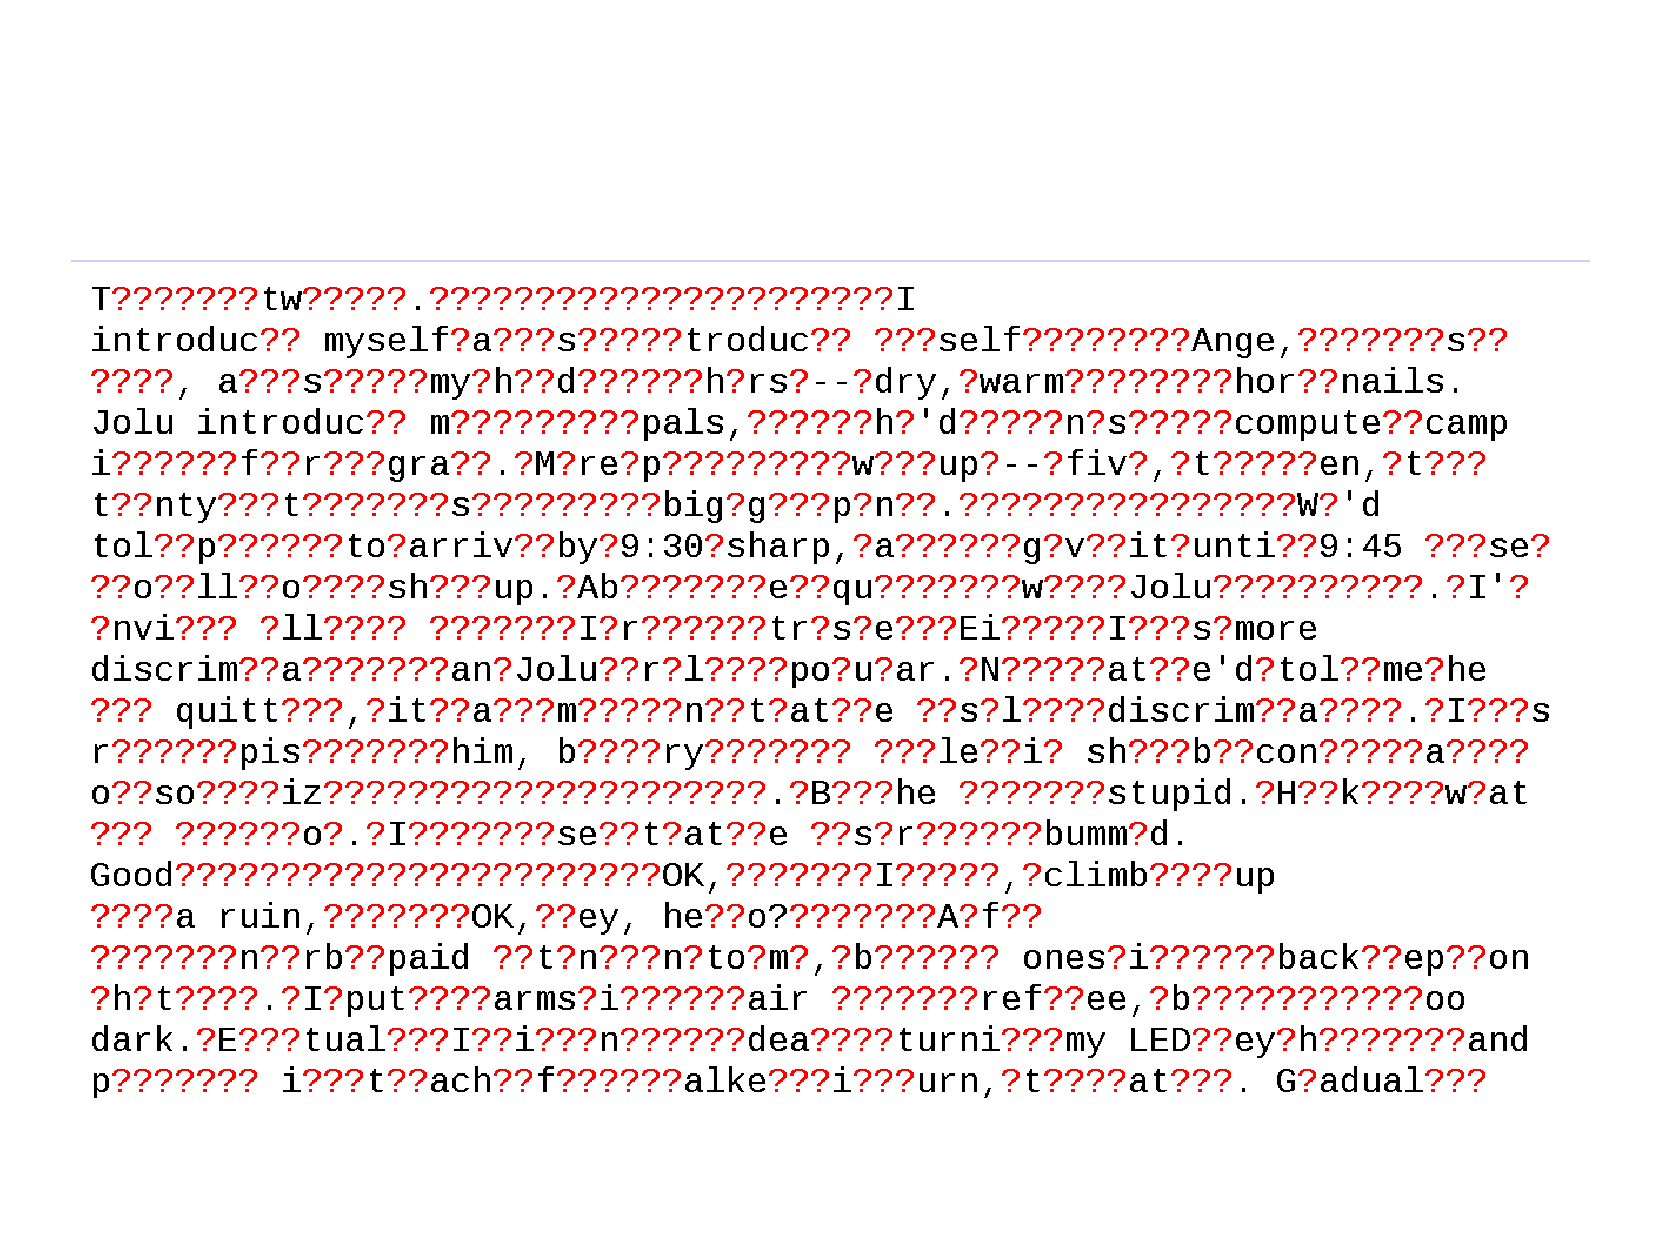
\includegraphics[width=3in]{art/brown-1} &  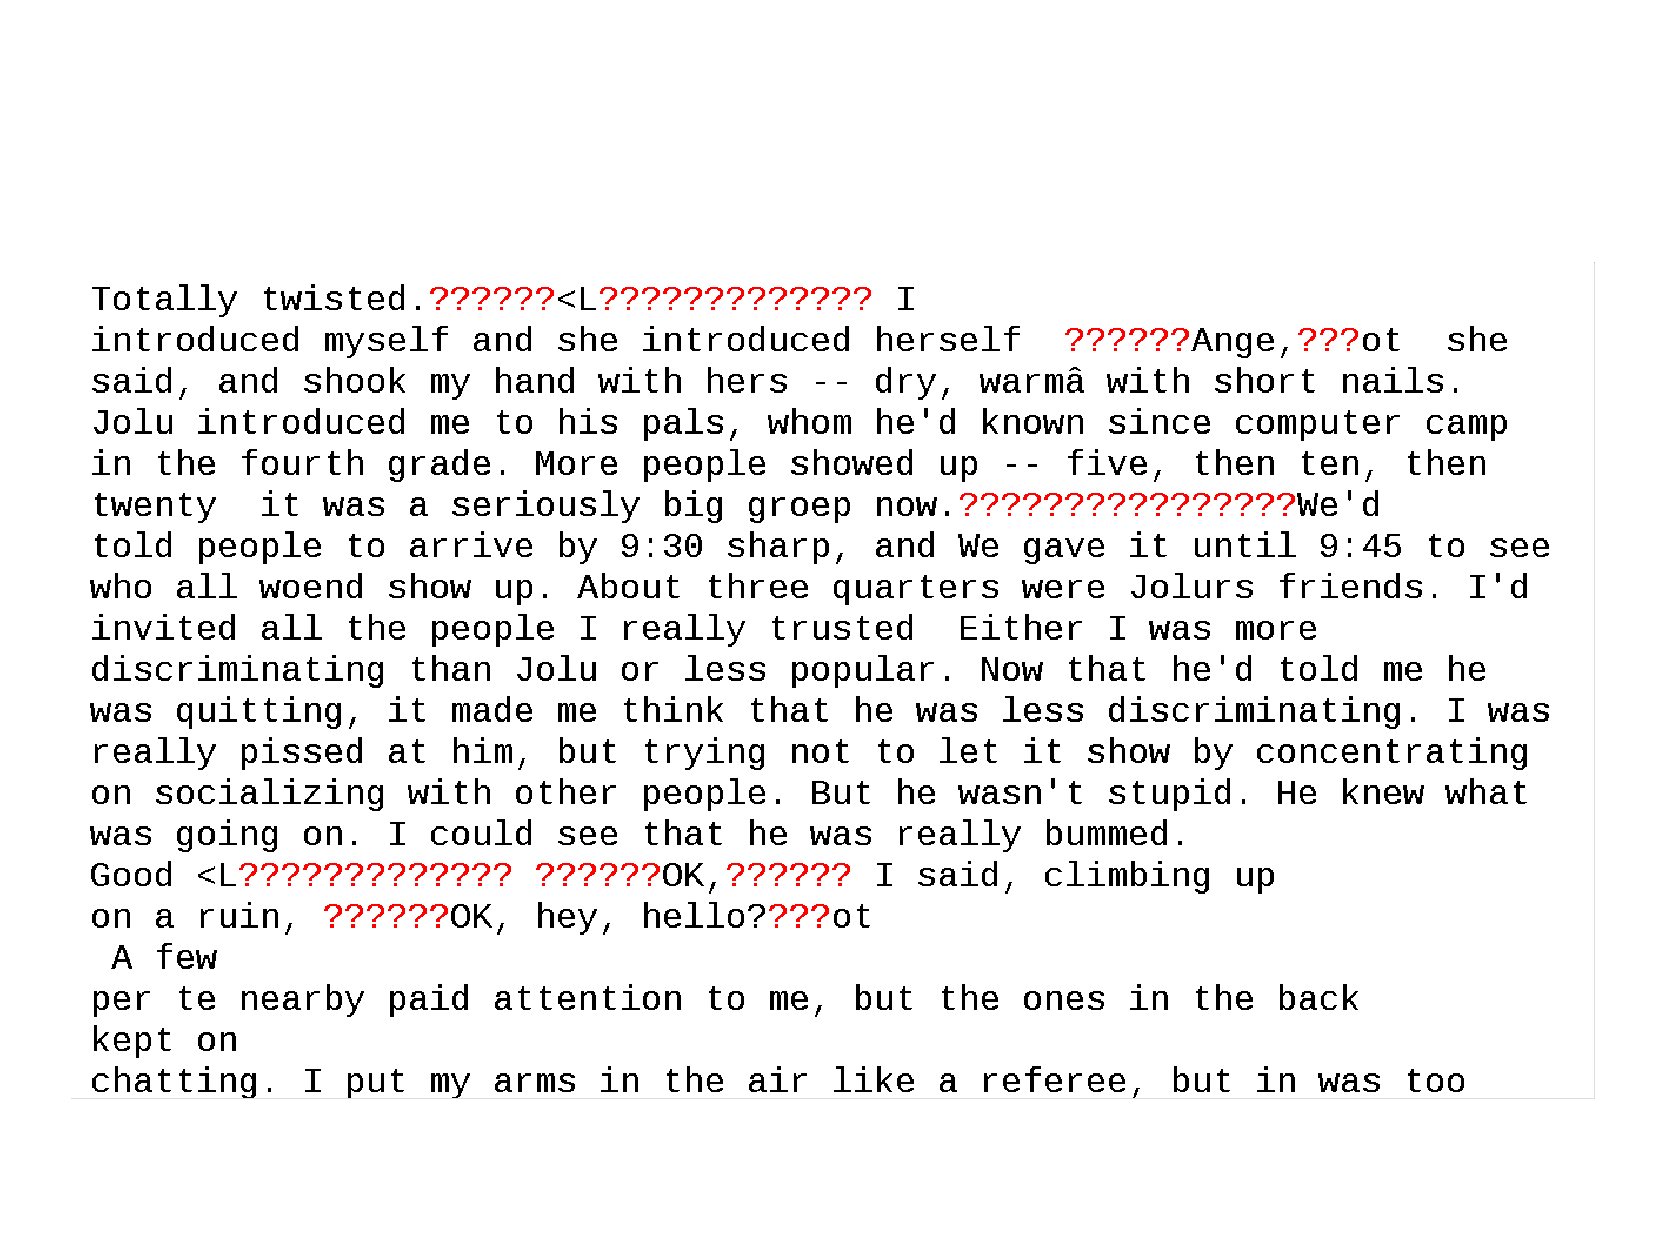
\includegraphics[width=3in]{art/brown-2} \\
\caption{Reconstructed text, without language model}\label{brown-1}
& \caption{Best possible reconstructed text, with language model}\label{brown-2}\\
\hline
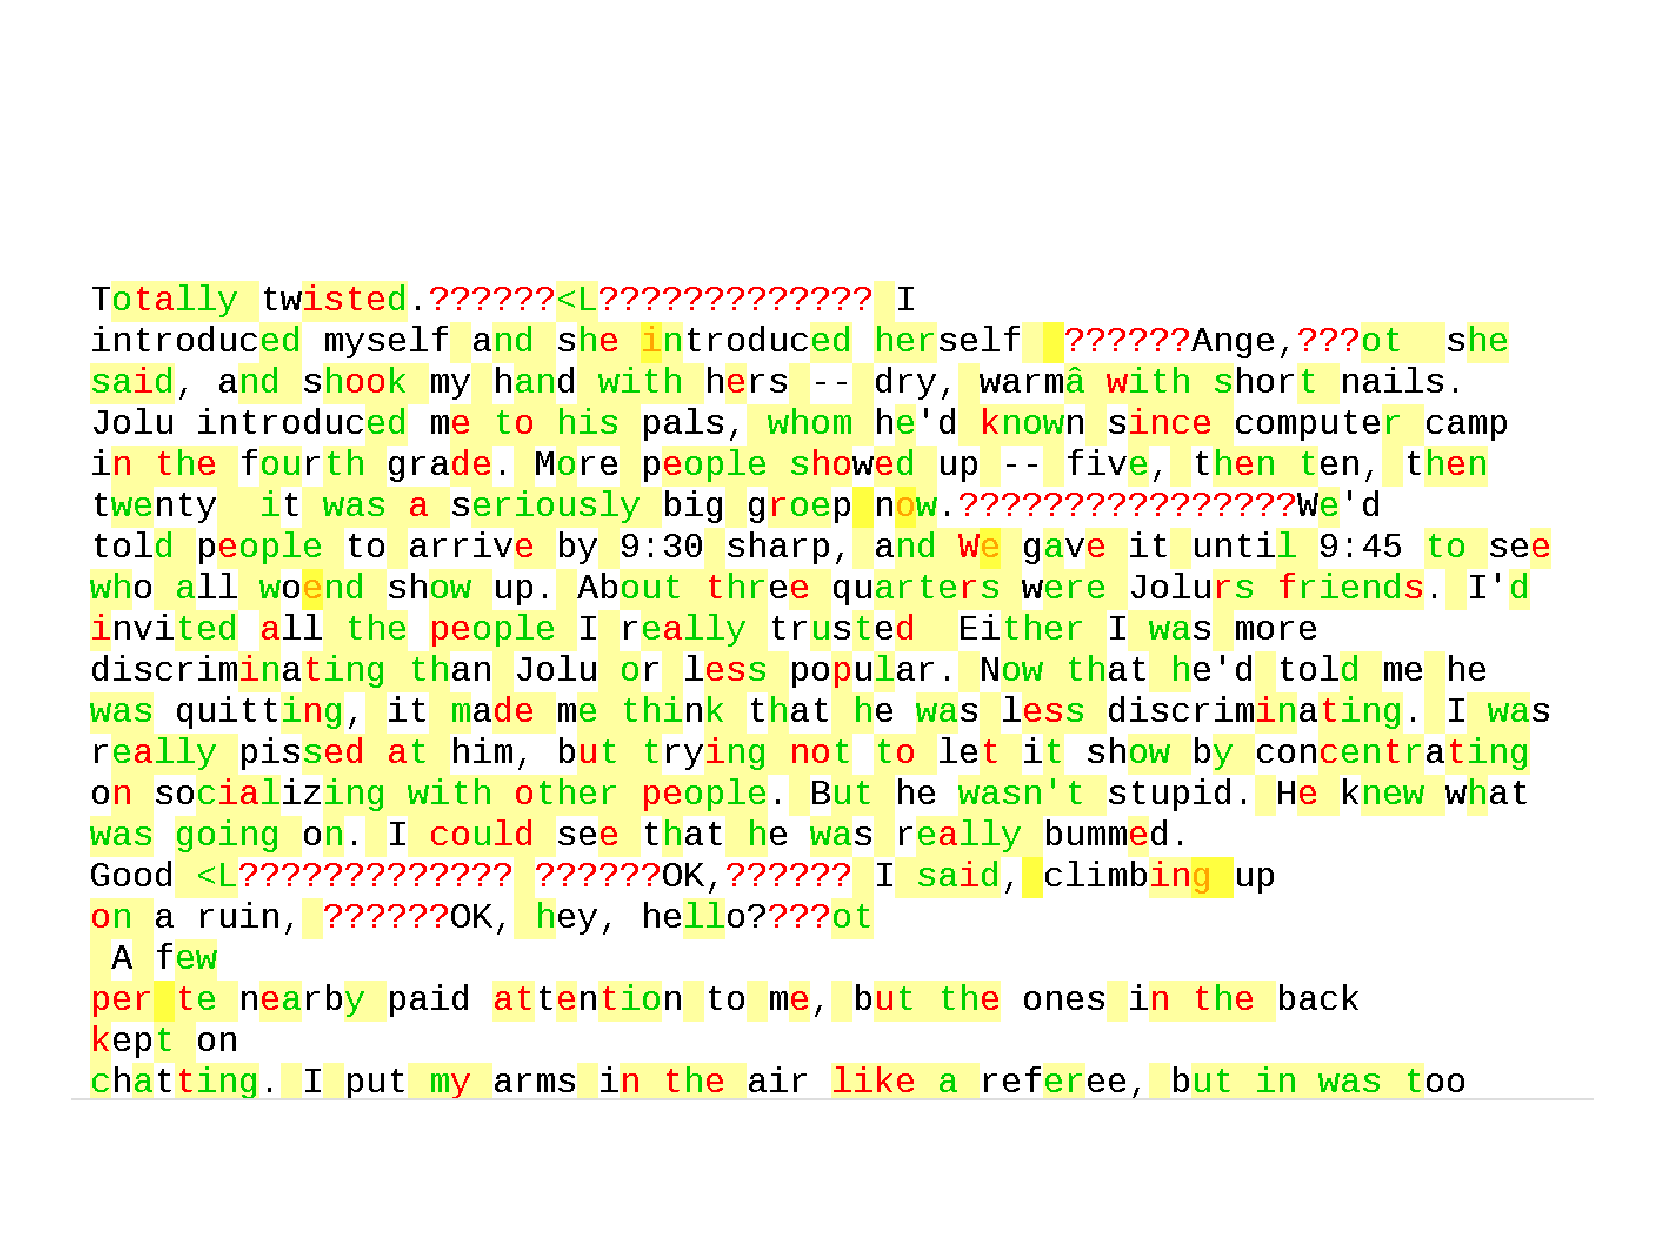
\includegraphics[width=3in]{art/brown-3} & 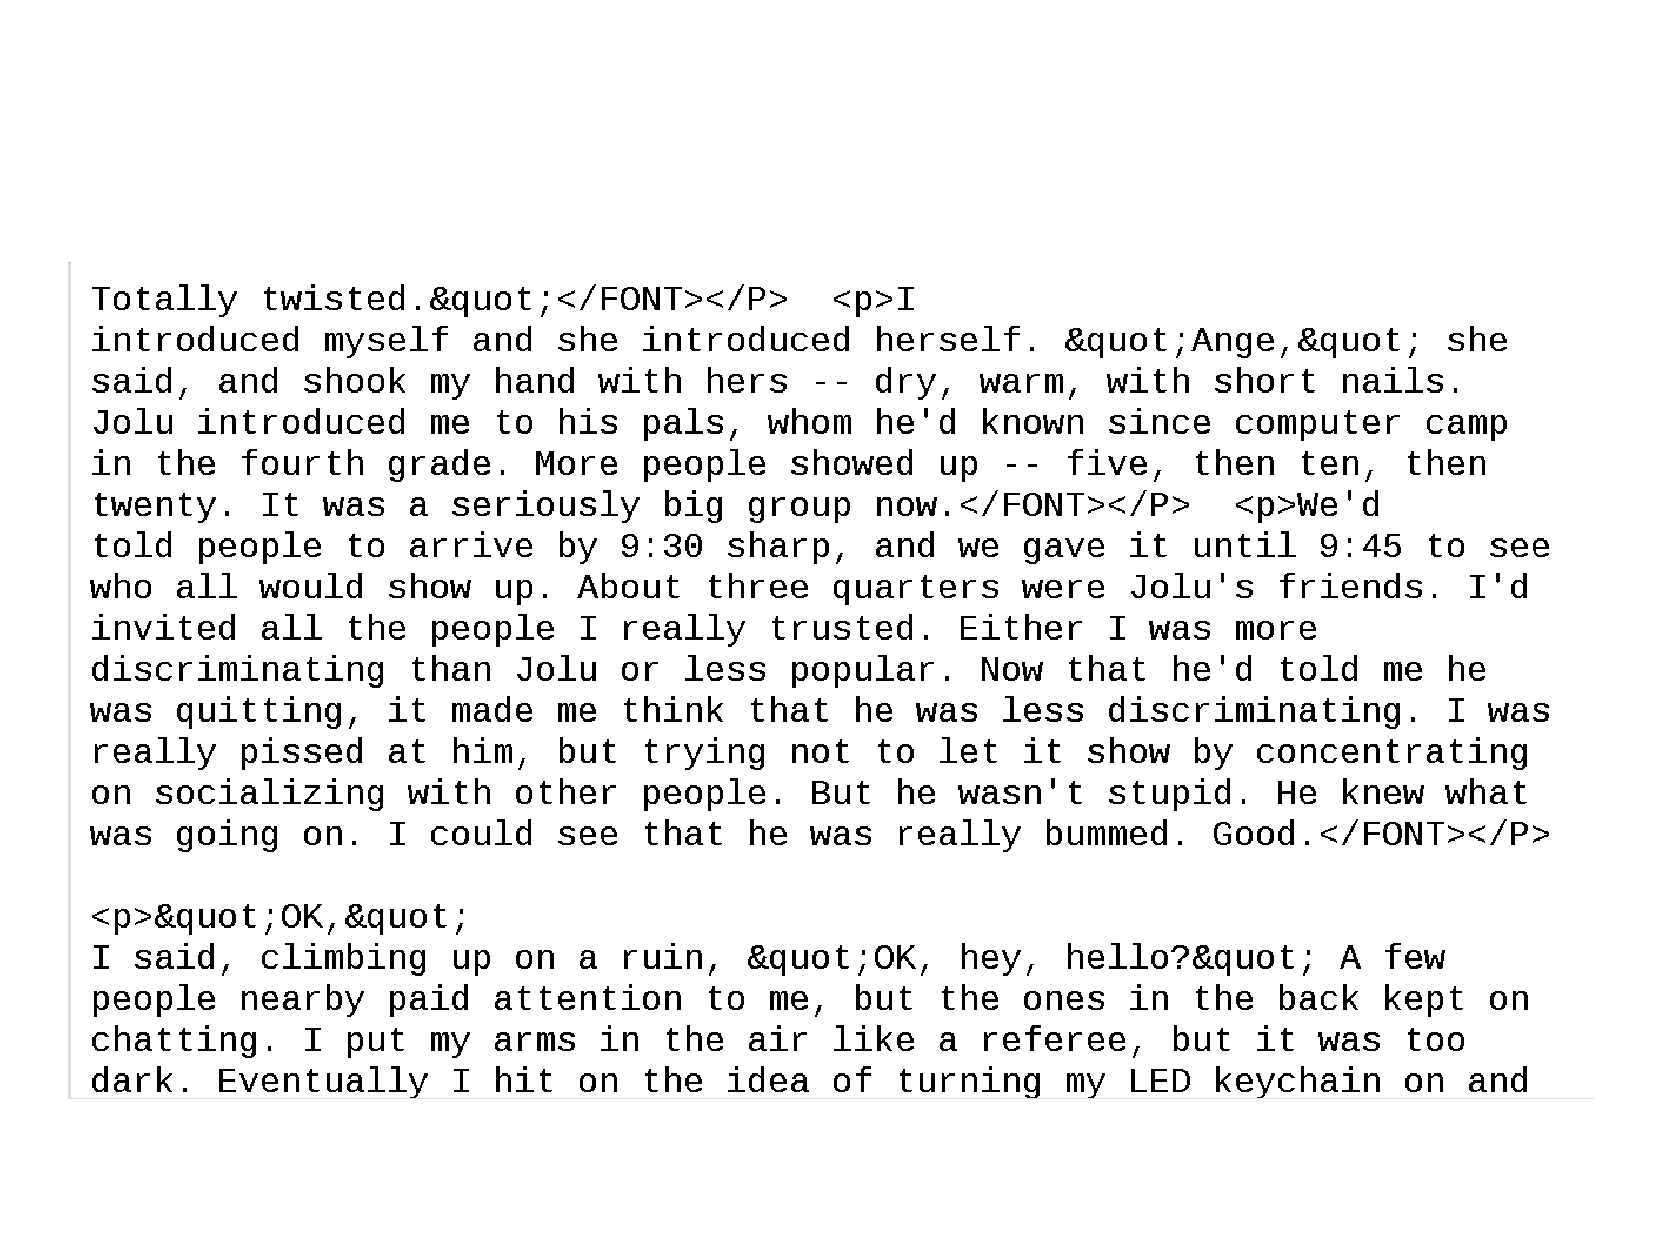
\includegraphics[width=3in]{art/brown-4}\\
\caption{Best possible reconstructed text, with language model. Green
  letters indicate high-probability matches, red letters indicate
  low-probability matches.}\label{brown-3}
&
\caption{Original text, from HTML version of Cory Doctorow novel
  ``Little Brother'', compressed using Info-Zip version 3.0, first
  1024 bytes of archive removed}\label{brown-4}
\\
\hline
\end{tabular}
\end{figure}


\subsection{Memory Parsing}

The memory of a desktop, laptop or cell phone is a mosaic of 4096-byte
blocks that variously 
contain running program code,  fragments of programs
that recently ran and have exited, portions of the computer's
operating system, fragments of what was sent and received over the
network, fragments of windows displayed on the computer's screen, the
computer's copy-and-paste buffer, and other kinds of information. Memory
changes rapidly---typical memory systems support several billion
changes per second---so it is nearly impossible to make a copy that is
internally consistent without halting the machine. An added complication is that the very
specific manner that programs store information in memory is rarely
documented and changes between one version of a program and
another. As a result, each version may need to be painstakingly reverse-engineered by
computer forensics researchers. Thus, memory analysis is time consuming, very
difficult, and necessarily incomplete.

Despite these challenges, recent years has seen the development of
forensically sound techniques for acquiring and analyzing the contents
of a running computer system. Today there are both open source and
proprietary memory analysis tools. These tools can take a memory dump
and report the system time when the memory was captured, display a
list of running processes, open files, and even display the contents
of the computer's clipboard and screen. Today memory analysis tools
are widely used for reverse-engineering computer viruses, worms and
other kinds of \emph{malware}, as well as for understanding an
attacker's actions in computer intrusion cases. Memory analysis can be combined
with carving to recover digital photographs and video.

\subsection{Fraud Detection in Multimedia}

Even when photos and video can be recovered from a subject's computer
or cell phone, another question to consider is whether or not the
imagery is real. Photographs were doctored long before the advent of
PhotoShop. For example, after he was purged by Stalin, Abel
Yenukidze was carefully removed from official photographs through a
series of skillful manipulations of light and negatives in a Kremlin darkroom\citet{stalins-darkroom}. Today
computer animation takes such manipulation to a completely new level,
with computers now able to synthesize scenes that are 
indistinguishable from recorded reality (\figref{ultra-realistic}). 

\begin{figure}
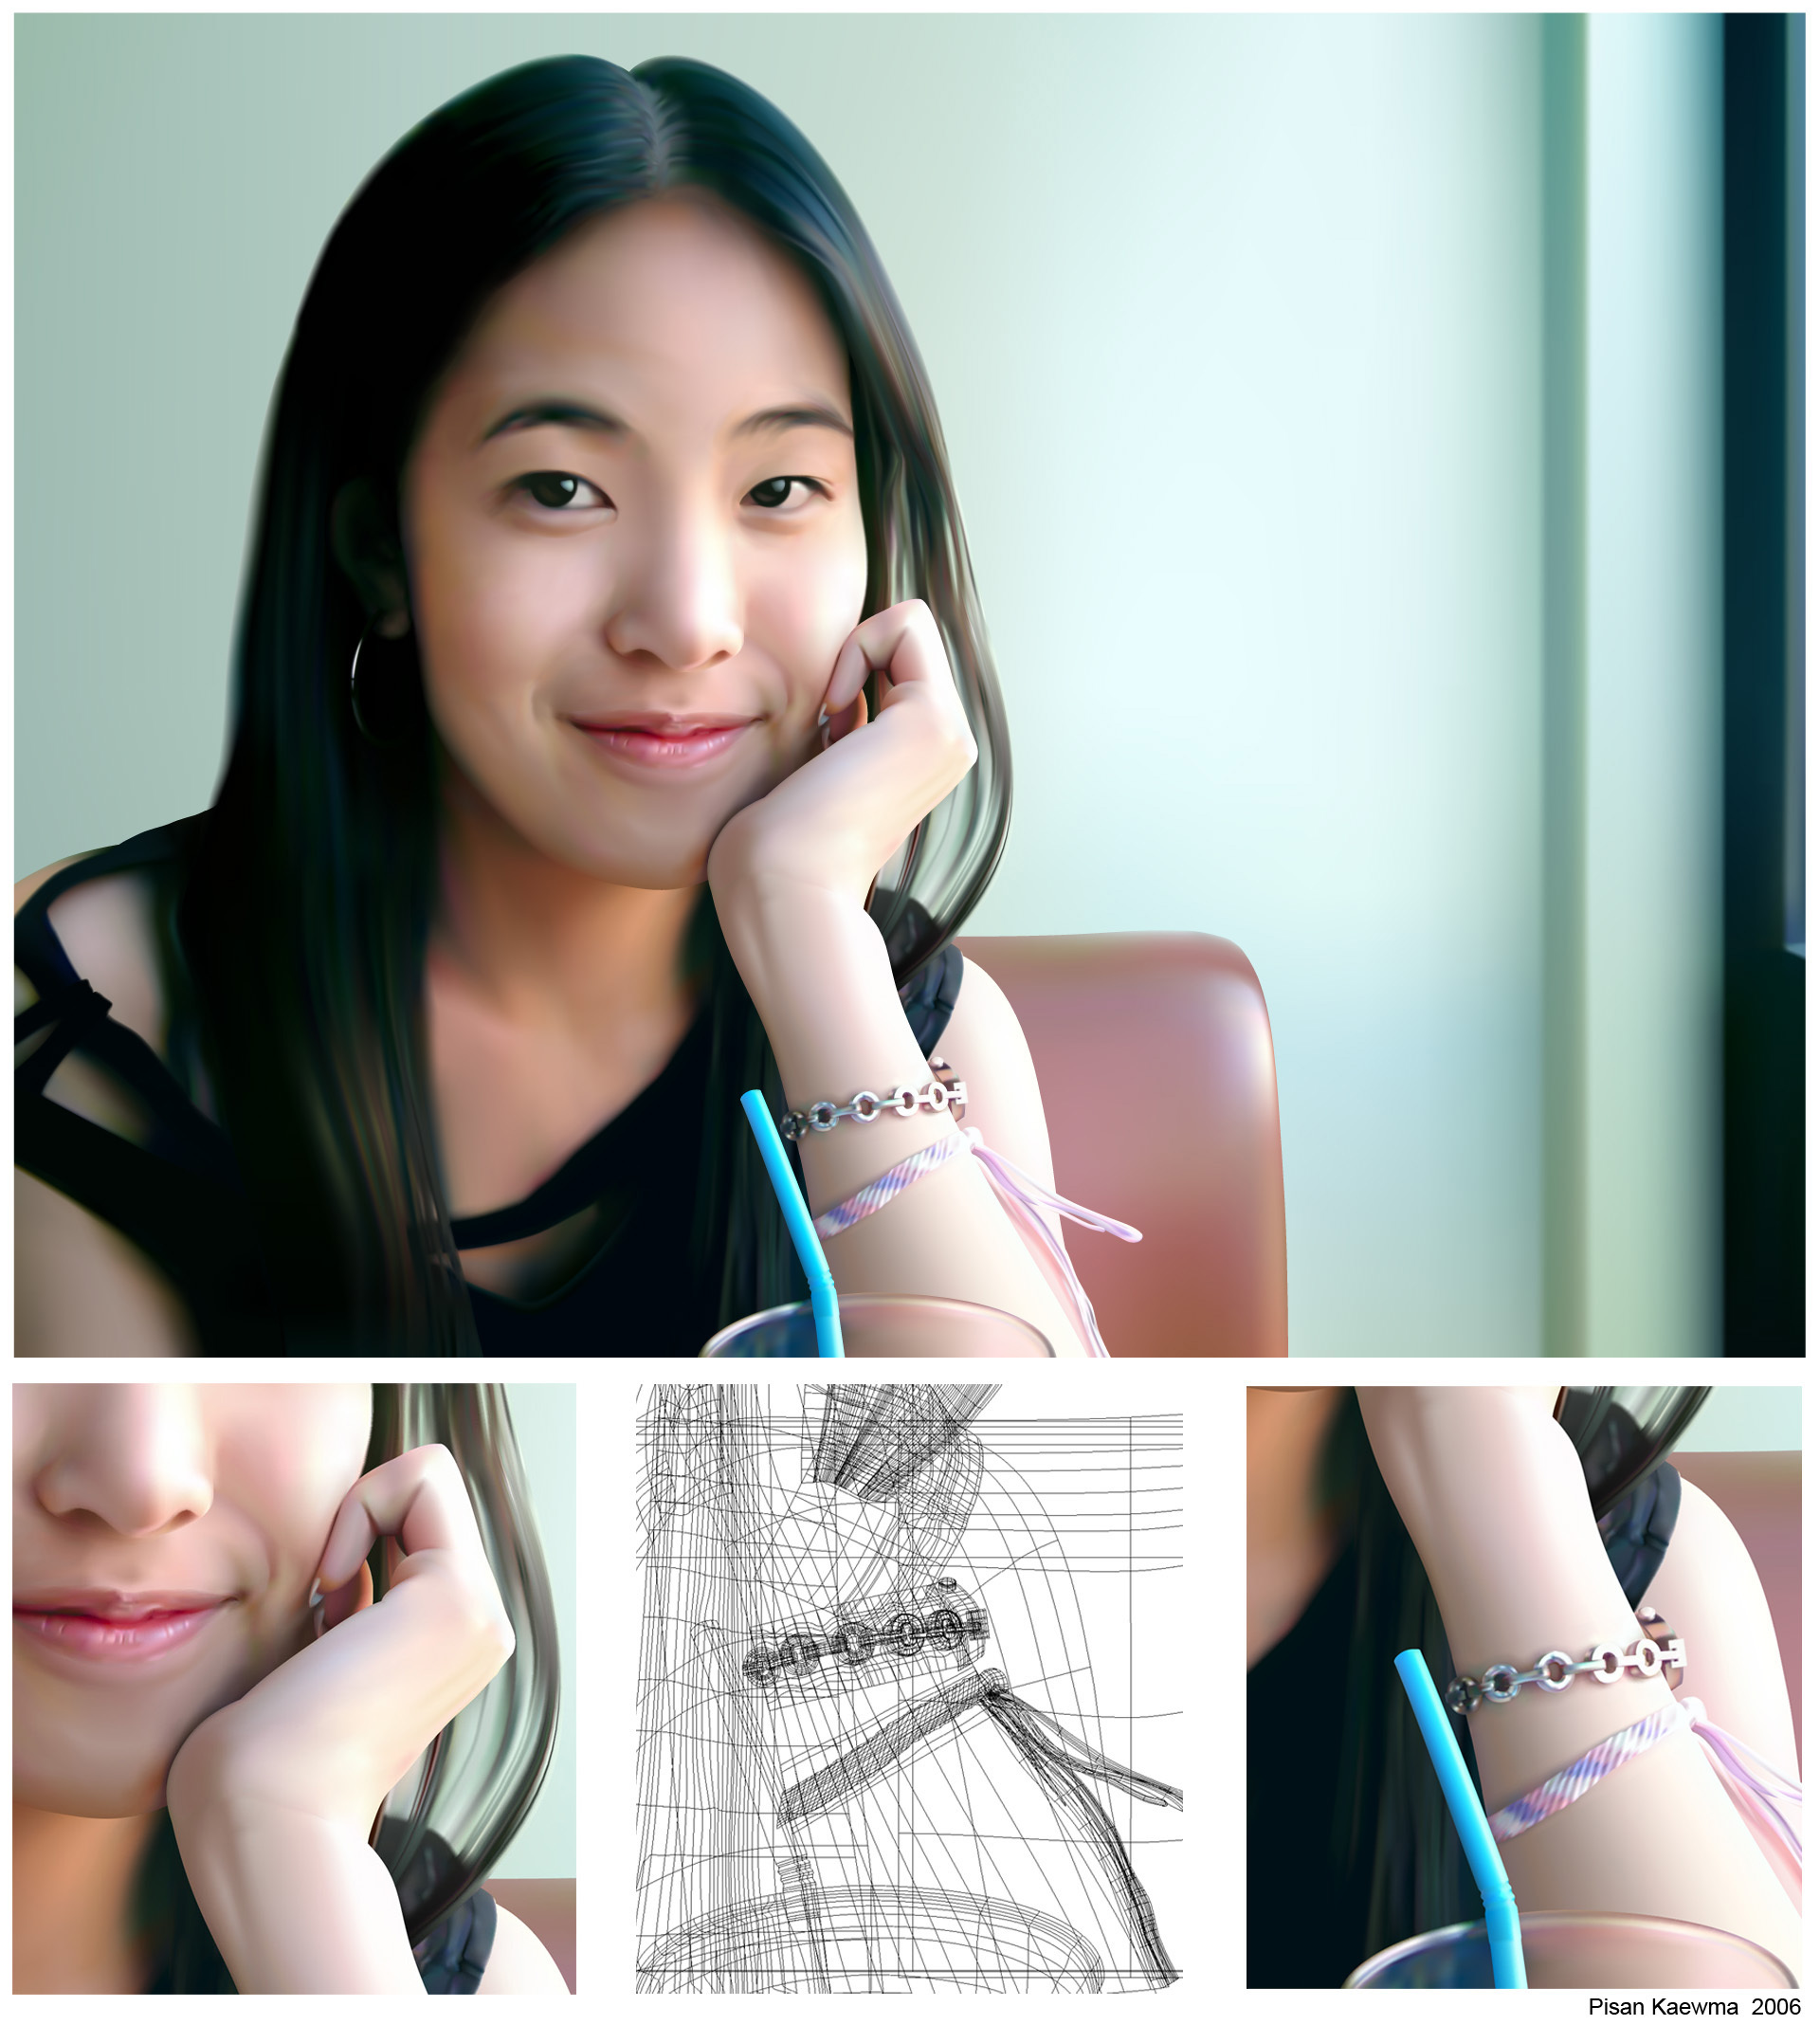
\includegraphics[width=4in]{art/a1336.jpg}
\caption{Ultra realistic vector gradient mesh using Adobe Illustrator by Pisan Kaewma, Thailand}\label{ultra-realistic}
% http://10steps.sg/inspirations/artworks/photo-realistic-vectors/
% http://www.ebypaidrick.com/Gallery.html
% http://www.illustratorworld.com/artwork/1336/
% http://rcpopart.com/labels/hyper-realist%20sculptor.html
% http://www.real-trace.com/index.html
\end{figure}

Recent developments in image processing have made it
possible to find some kinds of artifacts that indicate tampering or wholesale synthesis. For example,
the JPEG compression algorithm produces a mathematical signature when an
image is decompressed, cropped, and then re-compressed. Specular 
reflection, highlights and shadows can be closely examined to reveal
that different objects in a single ``photograph'' actually were
assembled from objects that were in 
slightly different physical environments. In one particular dramatic
demonstration, Dr.\ Hany Farid of Dartmouth University showed that a single ``group picture''
had been created by pasting in the people from different photos
because the reflection of the room lights on each person's eyeballs
were inconsistent with were they were standing in the frame. The technology is now
being commercialized\citep{farid07}.


\subsection{Automated Reasoning}

The leading edge of DF research are systems that
attempt to assist or even automate an analysts' reasoning---systems
that can automatically find evidence that is out of the ordinary,
strange, or inconsistent. Such details can indicate that there is a
deeper, hidden story. Inconsistencies can also indicate that evidence has been
tampered or entirely falsified. 

Ultimately, such automated reasoning systems are likely the only way
that today's analysts will be able to address the vast data
quantities and increasing diversity that they are likely to encounter
in the coming years. There has been some work in this area in
terms of systems that can find timestamp inconsistencies (a file
can't be deleted before it is created), but such rules are invariably
complicated by the messiness of the real world (for example, daylight
savings time). 

\section{The Digital Forensics Challenge}

For all of its power, DF practitioners face stark
challenges in practicing their discipline---challenges likely to
increase in the coming years. Those challenges are size,
time, diversity, cloud computing, encryption and language.

\begin{compactdesc}

\item[Size:] The past three decades have seen a steady increase in the
  amount of storage available to consumers and a steady decline in its
  cost. In 1993 I purchased my first 1 gigabyte external hard drive
  for a thousand dollars; today a 1 terabyte external hard drive can
  be purchased for under a hundred---a thousand times more
  storage for a tenth the price. Not surprisingly, the amount of data
  acquired by law enforcement organizations in their cases is
  increasing every year.

  Alarmingly, other aspects of computing have not scaled as quickly as
  storage. Today's terabyte drives are only 10 to 100 times faster
  than the gigabyte drives of yesteryear, which means that it takes anywhere
  from 10 to 100 times longer to copy  data from the larger
  drives. Likewise, today's computers are only on average 100 fold
  faster than the high-end workstations of the early 1990s, which
  means that there is less computing power available to process each
  byte per unit time. The continuation of these trends means that new techniques are
  required to deal with the data onslaught, as existing techniques
  simply cannot keep up with the increased storage available to consumers.

% My 33Mhz NeXTstation had 10 SPECmarks
% http://www.kevra.org/TheBestOfNext/NeXTProducts/NeXTHardware/NeXTStnColor/files/page620_2.pdf
% Intel Core i7 is 965 SPECmarks
% http://openlab.web.cern.ch/sites/openlab.web.cern.ch/files/technical_documents/CERN_openlab_report-Eval-of-energy-consumption-and-perf-of-Intel's-Nehalem-achitecture.pdf

\item[Time:] Even as the amount of storage received by law enforcement
  organizations increases, the time available to analyze that storage
  is steadily decreasing. In part this is because the number of cases
  in which digital evidence is collected is increasing far faster than
  the number of forensic investigators available to do the
  examinations. But another cause is the increasing realization that
  DF can be used to \emph{solve crimes}---that is, as
  part of the investigation process---whereas in the
  past DF was mainly a tool for \emph{assisting in convictions}. The
  shortened time horizons puts increased demands on tools,
  investigators, and systems.

\item[Diversity:] Forensic investigators must be able to process any
  information found on any computer system currently in use. After
  all, if there were a particular kind of system that could not be
  analyzed, criminals would be sure to use it. Thus, DF tools and
  invesitgators must be able to accommodate all kinds of computers,
  operating systems, application programs and the like. The diversity
  is particularly problematic in the case of cell phones, where there
  are literally dozens of different kinds of cables and tens of
  thousands of apps in widespread use that might require analysis.

\item[Cloud Computing:] Further complicating the investigator's job is
  the emergence of cloud computing and other technologies for storing
  data in the Internet rather than on desktops, laptops, and mobile
  devices. As a result of the cloud, there is no way to assure that a
  seized cell phone actually holds the suspect's data---the phone
  might simply be a tool for accessing a remote server. A law
  enforcement professional who is authorized to search a device may
  not have legal authority to use information on that device to access
  remotely stored data. Worse still, the data might be deleted in the
  meantime by one of the suspect's collaborators.

\item[Encryption:] The increased use of encryption means that
  investigators might not be able to decipher information once they
  have it in their possession. 

\item[Language:] Finally, in today's global environment forensics
  examiners are increasingly encountering evidence written in human
  languages that the examiner does not understand. And while tools
  like Systrans and Google Language Tools can perform some automated
  language translation, such systems are rarely sufficient for
  real-world forensic media.

\end{compactdesc}

These challenges impact the entire forensic processing model. Here are
two  examples:

\begin{compactitem}
\item Ten years ago it was relatively easy to collect and preserve a
computerized evidence: standard procedure was for law enforcement to
turn off a suspect's computer and take it back to the police station
where it might be put in an evidence locker. But modern computer systems
frequently employ encryption: turning them off may cause a key to be
erased, eliminating the possibility of decrypting the data without the
suspect's cooperation. For these systems it is now common practice to
copy out the computer's memory if possible---except that it is not
always possible because of diversity. 

\item Cell phones may be equipped with ``self destruct'' applications
  that wipe their data if they receive a particular text, so it is now
  standard practice to store phones in a shielded metal box called a
  Faraday cage that blocks radio waves. But many cell phones forget
  their storage if left off for too long, so the Faraday cages must be
  equipped with power strips and cell phone chargers.  Because many
  low-end cell phones have proprietary plugs, police must seize chargers as well.
\end{compactitem}


\subsection{The Research Agenda}

  Addressing these increases has only been possible through the
  collective research of government agencies, academics, and
  independent practitioners. These research efforts largely fall into
  three areas:

\begin{description}
\item[Reverse Engineering] has traditionally been the most basic form
  of DF research. Developers generally do not provide the public
  with details of how their systems work. This is obviously true of
  malware developers, but it is also true of legitimate companies that
  develop hardware and software, and even many open source
  systems. As a result, forensic practitioners must expend
  considerable effort reverse engineering systems to  understand how
  they work.  Today's techniques to extract allocated files from disk
  images were largely developed through reverse engineering.

\item[System Analysis] is the second leg of forensic research. System
  analysis is the systematic exploration of digital systems to
  understand the information that they contain and how it can be
  exploited for forensic analysis. Although similar to reverse
  engineering, system analysis is fundamentally different, in that the
  information the system analyst seeks may be unknown to the
  developers themselves. Although this may seem strange, remember that
  computers are vastly complicated systems: just as programmers
  frequently put bugs in their programs without realizing it, programs
  invariably have other behaviors that aren't bugs but are equally
  unforeseen by the original programmers. Many system users and quite
  a few developers assumed that it was not possible to recover deleted
  files until data recovery experts developed tools that proved otherwise.

 As long as there is data data that exists but which cannot be viewed
 through the operating system, there is need for tools that can
 display it. There is simply no commercial reason for software vendors
 to create tools which make this information visible---in many cases
 they are not even aware that the data is present. For example,
 previous versions of Microsoft Word left text in a
 document file even after it was deleted because the software didn't
 explicitly wipe the memory and corresponding disk sectors that
 corresponded to each deletion. This deleted-but-recoverable text
 occasionally resulted in some embarrassing revelations---so much, in
 fact, that many Microsoft products now explicitly have commands for
 to ``remove hidden data.'' Computer forensics tools can be
 used to both demonstrate the problem and verify whether or not
 Microsoft's solution actually works.

\item[Advances in fundamental science and engineering] are also needed
  for advances in DF. In particular, today's DF researchers are at the
  forefront of many other hot fields in computer science, including
  cloud computing, big data, visualization, and natural language
  processing. File carving and the recovery of data from corrupted
  compressed files are both examples of this kind of work: much of
  this work was thought to be computationally prohibitive until new
  mathematical algorithms were developed that proved
  otherwise. Another example is software that automatically translates
  posts on Facebook and Twitter from the subject's native tongue into
  a human language that the examiner can understand.
\end{description}


\subsection{The Biggest Challenge: Human Capital}

Despite its technical sophistication and reliance on the minutiae of
digital systems, the single biggest challenge facing digital forensics
practice today has a decidedly human dimension: the lack of qualified
people to serve as DF researchers and practitioners. But the human
resources problem faced in forensics is not merely the result of the
general tech shortage: the very nature of digital forensics makes our
human resources problem significantly harder than faced by other
disciplines. 

Because DF's mission is
to understand any data that might be stored on a computer
system, we need individuals that have knowledge
of both current and past computer systems, applications, and data
formats. We need generalists in a technological society that
increasingly rewards experts and specialization. 

This human resource problem is a bigger barrier to the
future of forensics than 
any technological problem that we have ever encountered. Whereas full
disk encryption might prevent a single hard drive from being
deciphered, the lack of skilled individuals can lead to backlogs of
months or longer---preventing evidence from even being collected.

One way to address this training problem is to look for opportunities
to modularize forensic problems so that experts in related fields can
make meaningful contributions. 

I believe that another approach is to show how the underlying
principles and current tools of digital forensics can be widely
applied throughout our society. This will increase the research of DF
tools and hopefully, as a result, increase the user base of the software.

For example, many of the tools of digital forensics can be used
for privacy auditing. That is, instead of using the tools to find
personal information that might be relevant to a case, businesses and
individuals can use the tools to look for the inappropriate presence of personal
information left behind because of bugs or oversight. (I am currently
writing a textbook on this topic.) Likewise, individuals can use tools
like file carvers to recover photographs that have been accidentally
deleted from digital cameras.

More generally, as our cars, street signs, communication systems,
electrical networks, building materials, and even companions are
increasingly computerized, digital forensics is likely to be one of
the only way for understanding these systems when they misbehave---or
when they are subverted. The increased computerization of our society
assures the continuing need for forensics capabilities and
practitioners. But without fundamentally new approaches for developing
these tools and capabilities, the difficulty and cost of forensic analysis is likely
to increase along with the ever-expanding data sizes and system
complexity. It's not just an arms race between investigators and the
criminals that they are hunting, but between the investigators and the
developers of tomorrow's computer systems.

\section{Terminology}
\begin{description}
\item[Allocated (files and sectors)] Allocated files are files that can be viewed through
  the operating system; allocated blocks are blocks that have been
  allocated to a specific file and will not be re-used by the
  operating system unless the contents are first relocated
  elsewhere. cf with \emph{deleted files}.
\item[Bit] A binary digit (0 or 1). The word ``bit'' was coined by
  John W.\ Turkey (1915-2000) while working at Bell Labs and first appeared in
  print in Claude Shannon's seminal 1948 article on information
  theory, \emph{A Mathematical Theory of Communication}. (Turkey also
  coined the word \emph{software}.) Abbreviated with a lower-case
  letter \emph{b}.
\item[Byte] An ordered set of bits used to represent the minimum
  amount of data that can be read or written to a computer memory at a
  time. Modern computers use 8-bit bytes, allowing for 256
  ($2^8$)possible values (typically 0 through 255 if the byte is
  interpreted as an unsigned number, or -128 through 127 if the byte
  is interpreted as a signed value.) Abbreviated with an upper-case
  letter \emph{B}.
\item[Compression] A mathematical process for reducing the size of a
  file or other digital object. Compression can be \emph{lossless} or
  \emph{lossy}. In Lossless compression the original file can be recovered by
  \emph{decompressing}, while with lossy compression information is
  lost and the exact original cannot be recovered. (However, lossless
  compression may have such high fidelity that a human being is unable
  to distinguish between the original and the decompressed objects.
\item[Deleted files] Files whose contents can be recovered but the
  sectors of which are not allocated.
\item[Digital Forensics] ``A branch of forensic science encompassing the
  recovery of and investigation of material
  found in digital devices, often in relation to computer crime.''\cite{reith:examination}
\item[Digital Trace Evidence] Another name for \emph{residual data}.
\item[Disk Image] A byte-for-byte copy of all the data on hard drive,
  camera card, or other kind of sector-oriented mass storage
  device. Disk images can contain additional metadata such as an
  embedded cryptographic hash of the original media, the date that the
  image was made, the examiner who made the image, as well as notes.
\item[Disk Imager] A program for making disk images.
\item[Media Exploitation] The extraction, translation and
  analysis of digital documents and media to generate
  useful and timely information.
\item[File] An ordered collection of 0 or more bytes. Files have a
  length; they may optionally metadata such one or more file names,
  modification dates, owners, and other information.
\item[File Header] One or more fixed bytes at the beginning of a
  file. For example, ZIP files begin with the file header ``PK'' (hex
  \texttt{50 4B}), while JPEG files begin with the field header
  \texttt{FF D8 FF E0}.
\item[File Footer] One or more fixed bytes at the end of a file. JPEG
  files end with the file footer \texttt{FF D9}.
\item[File System] Part of a computer's operating system which
  controls the storage of files on a mass storage system such as a
  hard drive or camera card.
\item[Forensic Science]
\item[Hash Value] Always say \emph{hash value}, never \emph{hash
  code}, since the word \emph{code} might refer to either the hash
  value or the program that computes the value.
\item[Investigator-Centric] Digital Forensics is said to be
  ``investigator-centric,'' meaning that most of the advances in the
  field have been to serve specific needs of investigators, rather
  than based on what is scientifically or technically possible.
\item[Logical Block Address (LBA)] \emph{Sectors} of a mass storage
  device are arranged in numbered sectors, starting with LBA 0. Early
  PC systems used hard drives that supported a 22-bit LBA and 512-byte sectors, allowing for a
  total of $2^{22}\times 2^{9}=2^{31}=2\textrm{TB}$ of storage. The
  current Advanced Technology Attachment standard, ATA-6, supports
  48-bit LBA addresses and a 4096-bit sector size, for a maximum disk
  with $2^{48}\times 2^{12}=2^{60}\approx 1,152,921\textrm{TB} \approx 1
  \textrm{EB (exabyte)}$ of storage.
\item[Malware] Software that embodies evil intent, such as to damage
  computer systems or steal private information. Computer Viruses,
  worms, and Trojan horses are examples of malware. 
\item[Metadata] Data about other data. The created, modified and
  access timestamps associated with a file on a camera card are
  examples of metadata.
\item[MD5] Message Digest \#5, a cryptographic hash algorithm
  developed by MIT professor Ron Rivest in 1991. Although MD5 is
  widely used in computer forensics, MD5 has known flaws and should
  not be used in applications that depend upon collision resistance.
% \item[Network forensic analysis tool (NFAT)] A system that can record
%   packets as they move over a network and perform detailed
%  after-the-fact analysis.
% \item[normalization]
% \item[Packet] A set of bytes that are sent over a network. Most
%   Internet packets range in size from 40--1500 bytes.
% \item[PCAP File] A packet capture file, which is typically a set of
%   packets that were recorded using a packet sniffer.
% \item[Packet sniffer] A program or device that can record packets are
%   they move over a network.
% \item[Packet Traces]
% \item[Provenance]
\item[Residual Data] data that is left behind on a computer after an
  operation is completed but is no longer in active use. For example,
  most computer systems erase the file name when a file is deleted,
  but do not overwrite the actual file contents. These contents remain
  on the drive as residual data, recoverable with computer forensic tools.
\item[Sector] The minimum amount of data that can be read or written
  to a mass storage device. Modern hard drives use sectors of 4096
  bytes; drives with 512-byte sectors have been common since the mid
  1970s and are still widely used today.
\item[Subject Computer and Data] The computer system and data that are
  being analyzed as part of a digital investigation. This may be data
  extracted from a computer belonging to a suspect in a crime, but it
  may also be data from the computer of a victim. Subject data may
  even be data generated during the course of a DF tool.
\item[Subject] is a common shorthand for the owner or primary use of a computer
  system from which subject data was obtained. 
\item[Tool-Based] Digital Forensics is said to be ``tool-based,''
  meaning that most investigators in their investigations to the
  capabilities provided by today's tools---investigators generally do
  not devise their own digital experiments or invent new approaches
  for working with data to solve specific cases.
\item[Timestamp]
\item[Unallocated sectors] Sectors that are not allocated to files or
  metadata, but are instead available for use by the file system
\end{description}


% LocalWords:  probative centric transformative Merkle combinatorial modularize
% LocalWords:  Ponzi Specular DF Madoff pre GPS Cyber imager
